\documentclass[12pt]{article}
\usepackage[T1]{fontenc}
\usepackage[spanish]{babel}
\usepackage{listings}
\usepackage{graphicx}
\graphicspath{ {./figuras/} }
\UseRawInputEncoding

\title{Proyecto Final de Informática}
\author{Julian Rodríguez Vega, Dayanna Lugo Vargas y Maria Fernanda Marin}
\date{Agosto 2021}

\begin{document}

\begin{titlepage}
\maketitle
\end{titlepage}

\section{Menú}

Iniciando con el menú de inicio, con un ciclo \verb+do while+ o un ciclo \verb+while+, junto a una variable de tipo booleana, es posible programar un programa por consola que pueda continuar corriendo constantemente.

\begin{lstlisting}[language=c++]
int main(){
    bool run = true;
    do {
        // Programa
    } while(run);
    return 0;
}
\end{lstlisting}

Dentro de este ciclo  sera necesario cambiar el valor de \verb+run+, para salir del ciclo y terminar la ejecución del programa.

\begin{figure}[h]
\caption{Diagrama de Flujo del Ciclo para un Menú}
\centering
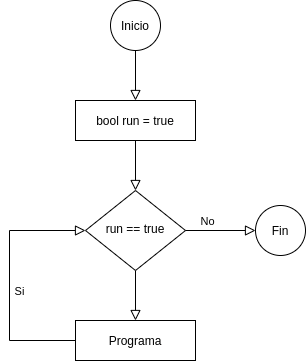
\includegraphics[scale=0.5]{menu_loop.png}
\end{figure}

Con una variable programa se captura que programa el usuario desea ejecutar, esta variable es evaluada con un switch envez de agrupar multiples condicionales.

\begin{lstlisting}[language=c++]

cout << "Programas Disponibles" << endl;
cout << "1. Calculador de Promedio" << endl;
cout << "2. Contador de Digitos." << endl;
cout << "3. Sucesión Numerica." << endl;

int programa;
cout << "Ingrese una opción: ";
cin >> programa;

switch(programa) {
    case 1:
        // Programa Calculador de promedio
        break;
    case 2:
        // Programa Contador de Digitos
        break;
    case 3:
        // Programa Susesión Numerica
        break;
    default:
        cout << "Esa no es una opción valida";
}
\end{lstlisting}

\end{document}
